%% usv_hydro -- Physical Models and Formulas Technical Report (English)
%% Compile: pdflatex usv_hydro_physics_report_en.tex (twice)
\documentclass[12pt,a4paper]{article}

%% -----------------------------------------------------------------------
%% PACKAGES
%% -----------------------------------------------------------------------
\usepackage[utf8]{inputenc}
\usepackage[T1]{fontenc}
\usepackage{lmodern}
\usepackage{microtype}

\usepackage[margin=2.5cm,top=3cm,bottom=3cm]{geometry}

\usepackage{amsmath,amssymb}
\usepackage{mathtools}
\usepackage{bm}

\usepackage{booktabs}
\usepackage{tabularx}
\usepackage{array}
\usepackage{longtable}
\usepackage{multirow}

\usepackage{graphicx}
\usepackage{xcolor}
\usepackage{float}
\usepackage{caption}

\usepackage{tikz}
\usetikzlibrary{shapes.geometric,arrows.meta,positioning,fit,backgrounds,calc}

\usepackage{listings}
\usepackage{courier}

\usepackage{hyperref}
\hypersetup{
  colorlinks=true,
  linkcolor=blue!60!black,
  pdftitle={usv\_hydro Physical Models Technical Report},
}

\usepackage{fancyhdr}
\pagestyle{fancy}
\fancyhf{}
\fancyhead[L]{\small \texttt{usv\_hydro} -- Physical Models Technical Report}
\fancyhead[R]{\small April 2026}
\fancyfoot[C]{\thepage}

%% -----------------------------------------------------------------------
%% LISTINGS
%% -----------------------------------------------------------------------
\definecolor{codebg}{RGB}{248,248,248}
\definecolor{codeframe}{RGB}{200,200,200}
\lstset{
  basicstyle=\small\ttfamily,
  backgroundcolor=\color{codebg},
  frame=single,
  rulecolor=\color{codeframe},
  breaklines=true,
  columns=fullflexible,
  keepspaces=true,
  showstringspaces=false,
}

%% -----------------------------------------------------------------------
%% SHORTCUTS
%% -----------------------------------------------------------------------
\newcommand{\nuvec}{\boldsymbol{\nu}}
\newcommand{\nudot}{\dot{\boldsymbol{\nu}}}
\newcommand{\xivec}{\boldsymbol{\xi}}
\newcommand{\Fvec}{\mathbf{F}}
\newcommand{\Kvec}{\mathbf{K}}
\newcommand{\Cvec}{\mathbf{C}}
\newcommand{\Avec}{\mathbf{A}}
\newcommand{\Bvec}{\mathbf{B}}
\newcommand{\Ainf}{\mathbf{A}(\infty)}

\renewcommand{\arraystretch}{1.35}

%% -----------------------------------------------------------------------
\begin{document}

%% ===========================  COVER  ===================================
\begin{titlepage}
  \centering
  \vspace*{2cm}
  {\Huge\bfseries usv\_hydro}\\[0.4em]
  {\Large\bfseries Physical Models and Formulas}\\[0.3em]
  {\large Technical Reference Report}
  \vspace{1.5cm}

  \rule{0.85\linewidth}{1pt}
  \vspace{0.5cm}

  \begin{tabular}{ll}
    \textbf{Project}  & Maritime Autonomous Systems Simulator \\
    \textbf{Package}  & \texttt{usv\_hydro} v0.1.0 \\
    \textbf{Platform} & ROS 2 Jazzy + Gazebo Sim 8 \\
    \textbf{Date}     & April 2026 \\
    \textbf{Status}   & Phase 1 Complete -- 21/21 tests passed \\
  \end{tabular}

  \vspace{1.5cm}\rule{0.85\linewidth}{0.4pt}\vspace{0.8cm}

  {\small This report provides a detailed description of each sub-model's
  input/output definitions, the physical formulas applied, configuration
  parameters, and inter-model data flow.}

  \vfill
  {\footnotesize Source files:\\
  \texttt{HydroTypes.cc}, \texttt{HydroCellSystem.cc},
  \texttt{BuoyancyModel.cc}, \texttt{DragModel.cc},
  \texttt{HydroIntegrator.cc}, \texttt{EnvironmentModel.cc}}
\end{titlepage}

\tableofcontents
\newpage

%% =======================================================================
\section{Introduction and System Architecture}
%% =======================================================================

\subsection{Overview}

\texttt{usv\_hydro} is a C++ physics plugin running on Gazebo Sim 8.
At each simulation step (\texttt{ISystemPreUpdate}) it reads body kinematics
from Gazebo, evaluates six physics sub-models, and injects the resulting
forces and moments back into the Gazebo physics engine via
\texttt{AddWorldWrench}.

\subsection{Inputs from Gazebo}

\begin{table}[H]
  \centering
  \caption{Input variables read from Gazebo at each step}
  \begin{tabularx}{\linewidth}{llX}
    \toprule
    \textbf{Variable} & \textbf{Type} & \textbf{Description} \\
    \midrule
    $\mathbf{p}_W$ & $\mathbb{R}^3$ & Body position in world frame (m) \\
    $\mathbf{q}_W$ & quaternion & World-frame orientation \\
    $\mathbf{v}^W$ & $\mathbb{R}^3$ & Linear velocity in world frame (m/s) \\
    $\boldsymbol{\omega}^W$ & $\mathbb{R}^3$ & Angular velocity in world frame (rad/s) \\
    $\Delta t$ & scalar & Simulation step duration (s) \\
    $t$ & scalar & Total simulation time (s) \\
    \bottomrule
  \end{tabularx}
\end{table}

The plugin derives body-frame velocity and acceleration:

\begin{align}
  \nuvec &= \begin{bmatrix}
    \mathbf{R}^T \mathbf{v}^W \\[2pt]
    \mathbf{R}^T \boldsymbol{\omega}^W
  \end{bmatrix} \in \mathbb{R}^6
  \label{eq:body_vel} \\[6pt]
  \nudot &\approx \frac{\nuvec(t) - \nuvec(t-\Delta t)}{\Delta t} \in \mathbb{R}^6
  \label{eq:body_accel}
\end{align}

where $\mathbf{R}$ is the world$\to$body rotation matrix (from $\mathbf{q}_W$).

\medskip
DOF ordering is consistent across all models:
\[
  [0{=}\text{surge},\;
   1{=}\text{sway},\;
   2{=}\text{heave},\;
   3{=}\text{roll},\;
   4{=}\text{pitch},\;
   5{=}\text{yaw}]
\]

\subsection{Total Force Composition}

Forces computed each step are applied via \texttt{AddWorldWrench}:

\begin{equation}
  \boxed{
  \Fvec_{\text{total}}
    = \Fvec_{\text{buoy}}
    + \Fvec_{\text{drag}}
    + \Fvec_{\text{stiff}}
    + \Fvec_{\text{rad}}
    + \Fvec_{\text{exc}}
  }
  \label{eq:force_sum}
\end{equation}

\subsection{Data-Flow Diagram}

\begin{figure}[H]
\centering
\begin{tikzpicture}[
  node distance=9mm and 16mm,
  blk/.style={rectangle, draw=blue!50, fill=blue!7, rounded corners=3pt,
              minimum width=4cm, minimum height=0.9cm,
              align=center, font=\small},
  inp/.style={rectangle, draw=orange!70, fill=orange!15, rounded corners=3pt,
              minimum width=5cm, minimum height=0.85cm,
              align=center, font=\small},
  out/.style={rectangle, draw=green!60!black, fill=green!10, rounded corners=3pt,
              minimum width=4.5cm, minimum height=0.85cm,
              align=center, font=\small},
  arr/.style={-{Stealth[length=2mm]}, thick, draw=blue!60},
]
\node[inp] (gz) {Gazebo kinematics\\
  $\mathbf{p}_W,\;\mathbf{q}_W,\;\mathbf{v}^W,\;\boldsymbol{\omega}^W,\;\Delta t,\;t$};
\node[blk, below left=12mm and 10mm of gz]  (env)  {EnvironmentModel\\
  $d_k = z_{wl} - z_{k,W}$};
\node[blk, below right=12mm and 10mm of gz] (grid) {HydroCellGrid\\
  $N_x \times N_y \times N_z$ cells};
\node[blk, below=12mm of env]  (buoy) {BuoyancyModel\\
  $F_b = \rho g V_{\text{cell}} s_k$};
\node[blk, below=12mm of grid] (drag) {DragModel\\
  $F_d = b_i v_i + \tfrac{1}{2}\rho C_d A |v_i| v_i$};
\node[blk, below=12mm of buoy] (inte) {HydroIntegrator\\
  sum over cells};
\node[blk, right=18mm of inte] (stif) {LinearStiffness $6\times6$\\
  $\mathbf{f} = -\alpha\,\Cvec\,\xivec$};
\node[blk, below=12mm of inte]  (seek) {LinearSeakeeping\\
  $F_{\text{exc}} = \sigma\,\text{Re}\{F_0 e^{i\omega t}\}$};
\node[blk, right=18mm of seek] (cumm) {CumminsRadiation\\
  $F_{\text{rad}} = -\Ainf\,\nudot - \int\Kvec\,\nuvec\,d\tau$};
\node[out, below=12mm of seek] (sum) {$\sum$ Force / Moment\\
  \texttt{AddWorldWrench}};
\draw[arr] (gz.south west) -- (env.north);
\draw[arr] (gz.south east) -- (grid.north);
\draw[arr] (env.south)  -- (buoy.north);
\draw[arr] (grid.south) -- (drag.north);
\draw[arr] (env.east)   -- (drag.west);
\draw[arr] (grid.west)  -- (buoy.east);
\draw[arr] (buoy.south) -- (inte.north);
\draw[arr] (drag.south west) -- (inte.north east);
\draw[arr] (inte.south) -- (seek.north);
\draw[arr] (inte.east)  -- (stif.west);
\draw[arr] (seek.east)  -- (cumm.west) node[above,font=\scriptsize,midway]{$B(\omega_n)$};
\draw[arr] (stif.south east) -- (sum.north east);
\draw[arr] (seek.south) -- (sum.north);
\draw[arr] (cumm.south) -- (sum.north east);
\end{tikzpicture}
\caption{System data flow: from Gazebo kinematics to force composition}
\label{fig:dataflow}
\end{figure}

\newpage
%% =======================================================================
\section{EnvironmentModel -- Environment Model}
%% =======================================================================

\subsection{Purpose}

\texttt{EnvironmentModel} provides the fluid environment parameters
to all other models. It is a static data layer -- loaded from configuration
and not recomputed each step.

\subsection{Parameters}

\begin{table}[H]
  \centering
  \caption{\texttt{EnvironmentModel} parameters}
  \begin{tabularx}{\linewidth}{llX}
    \toprule
    \textbf{Parameter} & \textbf{Default} & \textbf{Description} \\
    \midrule
    \texttt{water\_level} & 0.0 m & Calm water surface height (world Z) \\
    $\rho$ \texttt{fluid\_density} & 1000.0 kg/m$^3$ & Fluid density \\
    $g$ \texttt{gravity} & 9.81 m/s$^2$ & Gravitational acceleration \\
    \texttt{current\_velocity} & $(0,0,0)$ m/s & Current velocity in world frame \\
    \bottomrule
  \end{tabularx}
\end{table}

\subsection{Formulas}

\textbf{Cell centre depth:}
\begin{equation}
  d_k = z_{wl} - z_{k,W}
  \label{eq:depth}
\end{equation}
$d_k > 0$: cell is submerged. $d_k < 0$: cell is above water.

\textbf{Relative velocity (current effect):}
\begin{equation}
  \mathbf{v}_{rel}^W = \mathbf{v}_{\text{body}}^W - \mathbf{v}_{\text{current}}^W
  \label{eq:rel_vel}
\end{equation}

%% =======================================================================
\section{HydroCellGrid + HydroIntegrator -- Cell Grid System}
%% =======================================================================

\subsection{Grid Construction}

The axis-aligned bounding box (AABB) of the body is read from Gazebo and
divided into $N_x \times N_y \times N_z$ cells:

\begin{align}
  V_{\text{cell}} &= \frac{V_{\text{AABB}}}{N_x N_y N_z}
  \label{eq:cell_vol} \\[4pt]
  h_{\text{cell}} &\approx \frac{H_{\text{AABB}}}{N_z}
  \label{eq:cell_h}
\end{align}

Cell position in world frame:
\begin{equation}
  \mathbf{p}_{k}^W = \mathbf{p}_W + \mathbf{R}\,\mathbf{r}_{k}^{\text{body}}
  \label{eq:cell_pos}
\end{equation}

\subsection{Cell Kinematics}

Rigid-body cell velocity:
\begin{equation}
  \mathbf{v}_{k}^W = \mathbf{v}^W + \boldsymbol{\omega}^W \times
  (\mathbf{R}\,\mathbf{r}_{k}^{\text{body}})
  \label{eq:cell_vel}
\end{equation}

Body-frame relative velocity:
\begin{equation}
  \mathbf{v}_{rel,k}^{\text{body}}
    = \mathbf{R}^T\!\bigl(\mathbf{v}_{k}^W - \mathbf{v}_{\text{current}}^W\bigr)
  \label{eq:cell_rel_vel}
\end{equation}

For each cell, \texttt{BuoyancyModel} and \texttt{DragModel} are invoked;
forces are rotated to world frame and applied via \texttt{link.AddWorldForce(offset)}.

%% =======================================================================
\section{BuoyancyModel -- Buoyancy Model}
%% =======================================================================

\subsection{Purpose}

Computes the submerged volume fraction and resulting buoyancy force for
each cell, based on Archimedes' principle.

\subsection{Inputs}

\begin{table}[H]
  \centering
  \caption{\texttt{BuoyancyModel} inputs}
  \begin{tabularx}{\linewidth}{llX}
    \toprule
    \textbf{Input} & \textbf{Source} & \textbf{Description} \\
    \midrule
    $d_k$ & EnvironmentModel & Cell centre depth (m) \\
    $h_{\text{cell}}$ & HydroCellGrid & Cell height (m) \\
    $V_{\text{cell}}$ & HydroCellGrid & Cell volume (m$^3$) \\
    $\rho$ & HydroConfig & Fluid density (kg/m$^3$) \\
    $g$ & HydroConfig & Gravity (m/s$^2$) \\
    \bottomrule
  \end{tabularx}
\end{table}

\subsection{Formulas}

\textbf{Step 1 -- Submergence fraction:}
\begin{equation}
  \boxed{
  s_k = \mathrm{clamp}\!\left(\frac{d_k}{h_{\text{cell}}} + 0.5,\; 0,\; 1\right)
  }
  \label{eq:submergence}
\end{equation}

\begin{itemize}
  \item $s_k = 0$: cell fully above water
  \item $s_k = 1$: cell fully submerged
  \item $0 < s_k < 1$: free surface passes through cell
\end{itemize}

\textbf{Step 2 -- Submerged volume:}
\begin{equation}
  V_{\text{sub},k} = V_{\text{cell}} \cdot s_k
  \label{eq:sub_vol}
\end{equation}

\textbf{Step 3 -- Buoyancy force (Archimedes):}
\begin{equation}
  \boxed{F_{b,k}^z = \rho\, g\, V_{\text{cell}}\, s_k}
  \label{eq:buoyancy}
\end{equation}

Force direction is $+z$ only: $\mathbf{F}_{b,k}^W = (0,\,0,\,F_{b,k}^z)$.

\textbf{Total buoyancy force and moment:}
\begin{align}
  \Fvec_{\text{buoy}}^W &= \sum_{k:\,s_k>0} \mathbf{F}_{b,k}^W
  \label{eq:total_buoy} \\[4pt]
  \boldsymbol{\tau}_{\text{buoy}}^W &= \sum_{k:\,s_k>0} \mathbf{r}_k^W \times \mathbf{F}_{b,k}^W
  \label{eq:total_buoy_moment}
\end{align}

\textbf{Equilibrium condition:}
\begin{equation}
  \rho\,g\,V_{\text{disp}} = m\,g
  \quad\Rightarrow\quad
  V_{\text{disp}} = \frac{m}{\rho}
  \label{eq:equilibrium}
\end{equation}

\subsection{Numerical Values (Reference Vessel)}

\begin{table}[H]
  \centering
  \caption{Buoyancy model parameters for the reference USV}
  \begin{tabular}{llr}
    \toprule
    \textbf{Quantity} & \textbf{Formula} & \textbf{Value} \\
    \midrule
    Hull dimensions & $L \times B \times D$ & $2.2\times 1.1\times 0.5$ m \\
    Grid & $N_x\times N_y\times N_z$ & $14\times 8\times 4 = 448$ cells \\
    Cell volume & $V/N$ & $5.45\times10^{-4}$ m$^3$ \\
    Cell height & $H/N_z$ & 0.125 m \\
    Waterplane area & $L\times B$ & 2.42 m$^2$ \\
    Static draft & $m/(\rho L B)$ & $\approx 0.145$ m \\
    \bottomrule
  \end{tabular}
\end{table}

%% =======================================================================
\section{DragModel -- Viscous Resistance Model}
%% =======================================================================

\subsection{Purpose}

Computes viscous resistance from the fluid for each submerged cell,
including both linear and quadratic (Morison) terms.

\subsection{Inputs}

\begin{table}[H]
  \centering
  \caption{\texttt{DragModel} inputs}
  \begin{tabularx}{\linewidth}{llX}
    \toprule
    \textbf{Input} & \textbf{Source} & \textbf{Description} \\
    \midrule
    $\mathbf{v}_{rel,k}^{\text{body}}$ & HydroIntegrator & Body-frame relative velocity (m/s) \\
    $A_{\text{cell},i}$ & HydroCellGrid & Cell cross-section area in direction $i$ (m$^2$) \\
    $b_i$ & HydroConfig & Linear damping coefficient [N$\cdot$s/m] \\
    $C_{d,i}$ & HydroConfig & Quadratic drag coefficient [--] \\
    $s_k$ & BuoyancyModel & Submergence fraction $[0,1]$ \\
    $\rho$ & HydroConfig & Fluid density (kg/m$^3$) \\
    \bottomrule
  \end{tabularx}
\end{table}

\subsection{Formulas}

For $i \in \{\text{surge, sway, heave}\}$:

\begin{equation}
  \boxed{
  F_{d,i,k}^{\text{body}}
    = \underbrace{-b_i\,v_{rel,i,k}}_{\text{linear}}
    \;-\;
    \underbrace{\tfrac{1}{2}\rho\,C_{d,i}\,A_{\text{cell},i}\,
      |v_{rel,i,k}|\,v_{rel,i,k}}_{\text{quadratic (Morison)}}
  }
  \label{eq:drag}
\end{equation}

Scaling for partially submerged cells:
\begin{equation}
  F_{d,i,k}^{\text{eff}} = F_{d,i,k}^{\text{body}} \cdot s_k
  \label{eq:drag_scaled}
\end{equation}

Rotation to world frame:
\begin{equation}
  \mathbf{F}_{d,k}^W = \mathbf{R}\;\mathbf{F}_{d,k}^{\text{eff}}
  \label{eq:drag_world}
\end{equation}

\subsection{Profile Parameters}

\begin{table}[H]
  \centering
  \caption{Damping parameters across configuration profiles}
  \begin{tabular}{lccc}
    \toprule
    \textbf{Profile} & $b_x$ [N$\cdot$s/m] & $b_y$ & $b_z$ \\
    \midrule
    \texttt{baseline}      & 18  & 55  & 80  \\
    \texttt{low\_damping}  &  6  & 18  & 25  \\
    \texttt{high\_damping} & 30  & 90  & 130 \\
    \bottomrule
  \end{tabular}
  \par\smallskip
  {\small $C_{d,x}=0.9$, $C_{d,y}=1.3$, $C_{d,z}=2.0$ across all profiles.}
\end{table}

%% =======================================================================
\section{LinearStiffness6x6 -- Hydrostatic Stiffness Matrix}
%% =======================================================================

\subsection{Purpose}

Computes restoring forces and moments opposing the vessel's deviation
from its equilibrium position, expressed as a full $6\times6$ stiffness
matrix.

\subsection{6x6 Stiffness Matrix -- Finite Differences}

At the first simulation step, the reference pose
$(\mathbf{p}_{\text{ref}}, \mathbf{q}_{\text{ref}})$ is recorded.
For each DOF $j\in\{0,\ldots,5\}$ a $\pm$ perturbation is applied and
buoyancy forces are rotated to body frame:

\begin{equation}
  \mathbf{F}^{\text{body}}(\pm\Delta\xi_j)
    = \mathbf{R}_{\text{ref}}^T\;\mathbf{F}^{\text{world}}(\pm\Delta\xi_j)
  \label{eq:stiffness_fd}
\end{equation}

Central finite difference stiffness coefficient:
\begin{equation}
  \boxed{
  C_{ij} = -\frac{F_i^{\text{body}}(+\Delta\xi_j)
             - F_i^{\text{body}}(-\Delta\xi_j)}{2\,\Delta\xi_j}
  }
  \label{eq:c_matrix}
\end{equation}

\begin{table}[H]
  \centering
  \caption{Per-column perturbation vectors ($\Delta s$: translational step,
           $\Delta a$: angular step)}
  \begin{tabular}{clc}
    \toprule
    \textbf{Column $j$} & \textbf{DOF} & \textbf{Step size} \\
    \midrule
    0 & surge  & $\Delta s = 0.01$ m \\
    1 & sway   & $\Delta s$ \\
    2 & heave  & $\Delta s$ \\
    3 & roll   & $\Delta a = 10^{-3}$ rad \\
    4 & pitch  & $\Delta a$ \\
    5 & yaw    & $\Delta a$ \\
    \bottomrule
  \end{tabular}
\end{table}

\subsection{Restoring Wrench Computation}

Instantaneous 6-DOF displacement relative to reference pose:
\begin{equation}
  \xivec =
  \begin{bmatrix}
    \mathbf{R}_{\text{ref}}^T(\mathbf{p}^W - \mathbf{p}_{\text{ref}}) \\[2pt]
    \phi_e,\;\theta_e,\;\psi_e
  \end{bmatrix} \in \mathbb{R}^6
  \label{eq:xi}
\end{equation}

\begin{equation}
  \boxed{
  f_i^{\text{body}} = -\alpha \sum_{j=0}^{5} C_{ij}\,\xi_j,
  \quad i=0,\ldots,5
  }
  \label{eq:restoring}
\end{equation}

World-frame transformation:
\begin{equation}
  \Fvec_{\text{rest}}^W = \mathbf{R}_{\text{ref}}\,\mathbf{f}_{0:2}^{\text{body}},
  \qquad
  \boldsymbol{\tau}_{\text{rest}}^W = \mathbf{R}_{\text{ref}}\,\mathbf{f}_{3:5}^{\text{body}}
  \label{eq:restoring_world}
\end{equation}

\subsection{Analytical Comparison}

\begin{align}
  C_{33} &= \rho\,g\,A_{wp}
  &\text{(waterplane stiffness)} \label{eq:c33} \\
  C_{44} &= \rho\,g\,V\,\overline{GM}_T
  &\text{(roll restoring)} \label{eq:c44} \\
  C_{55} &= \rho\,g\,V\,\overline{GM}_L
  &\text{(pitch restoring)} \label{eq:c55}
\end{align}

\begin{table}[H]
  \centering
  \caption{Stiffness matrix validation results}
  \begin{tabular}{lccc}
    \toprule
    \textbf{Term} & \textbf{Analytical} & \textbf{Numerical} & \textbf{Error} \\
    \midrule
    $C_{33}$ & 23\,738 N/m & 23\,740 N/m & $<0.01\%$ \\
    $C_{44}$ & 1\,771 Nm/rad & 1\,771 Nm/rad & $<0.01\%$ \\
    $C_{55}$ & 8\,941 Nm/rad & 8\,941 Nm/rad & $<0.01\%$ \\
    $C_{11},\,C_{22}$ & $\approx 0$ & $\approx 0$ & -- \\
    $C_{35} \approx C_{53}$ & reciprocity & $<150$ Nm/m & -- \\
    \bottomrule
  \end{tabular}
\end{table}

%% =======================================================================
\section{LinearSeakeepingModel -- Frequency-Domain Seakeeping}
%% =======================================================================

\subsection{Governing Equation}

\begin{equation}
  \boxed{
  \Fvec_{\text{sk}}
    = \underbrace{-\Avec(\omega)\,\nudot}_{\text{added mass}}
    \;-\; \underbrace{\Bvec(\omega)\,\nuvec}_{\text{radiation damping}}
    \;+\; \underbrace{\text{Re}\!\left\{\Fvec_{\text{exc}}(\omega)\,e^{i\omega t}\right\}}_{\text{wave excitation}}
  }
  \label{eq:seakeeping}
\end{equation}

Excitation term in explicit form:
\begin{equation}
  F_{\text{exc},i}(t)
    = \sigma\!\left[F_{\text{exc},i}^{\text{Re}}\cos(\omega t)
      - F_{\text{exc},i}^{\text{Im}}\sin(\omega t)\right]
  \label{eq:excitation}
\end{equation}

\subsection{Inputs}

\begin{table}[H]
  \centering
  \caption{Seakeeping model inputs}
  \begin{tabularx}{\linewidth}{llX}
    \toprule
    \textbf{Input} & \textbf{Source} & \textbf{Description} \\
    \midrule
    YAML coefficient file & Disk & $\Avec(\omega_n)$, $\Bvec(\omega_n)$, $\Fvec_{\text{exc}}(\omega_n)$ \\
    $\omega$ & scalar & Evaluation frequency (rad/s) \\
    $\nuvec$ & HydroCellSystem & Body-frame 6-DOF velocity \\
    $\nudot$ & HydroCellSystem & Body-frame 6-DOF acceleration \\
    $t$ & Gazebo & Simulation time (s) \\
    $\sigma$ & scalar & Wave amplitude scaling factor \\
    \bottomrule
  \end{tabularx}
\end{table}

\subsection{YAML Coefficient Format}

\begin{lstlisting}
schema_version: 1
# DOF order: [surge, sway, heave, roll, pitch, yaw]
frequencies:
  - omega: 0.5             # rad/s
    added_mass:            # 6x6 matrix [kg]
      - [120.0, 0.0, 0.0, 0.0, 0.0, 0.0]
      ...
    damping:               # 6x6 [N*s/m]
      - [45.0, ...]
      ...
    excitation_re: [Fx, Fy, Fz, Mx, My, Mz]   # [N] or [N*m]
    excitation_im: [...]
  - omega: 1.0
    ...
\end{lstlisting}

Compatible with AQWA, Nemoh, or WAMIT outputs after conversion.

\subsection{Linear Interpolation}

\begin{equation}
  \alpha = \frac{\omega - \omega_{lo}}{\omega_{hi} - \omega_{lo}},
  \qquad
  \Avec(\omega) = (1-\alpha)\,\Avec(\omega_{lo}) + \alpha\,\Avec(\omega_{hi})
  \label{eq:interp}
\end{equation}

\subsection{Operating Mode Selection}

\begin{itemize}
  \item \textbf{Legacy mode} (\texttt{cummins\_radiation: false}):
        Full Equation~\eqref{eq:seakeeping} applied.
  \item \textbf{Cummins mode} (\texttt{cummins\_radiation: true}):
        Only the excitation term is computed; the radiation part
        is replaced by \texttt{CumminsRadiationModel}.
\end{itemize}

%% =======================================================================
\section{CumminsRadiationModel -- Time-Domain Radiation Model}
%% =======================================================================

\subsection{Cummins Equation}

\begin{equation}
  \boxed{
  \bigl[\mathbf{M} + \Ainf\bigr]\,\nudot(t)
  + \int_0^t \Kvec(t-\tau)\,\nuvec(\tau)\,d\tau
  + \Cvec\,\xivec(t)
  = \Fvec_{\text{exc}}(t) + \Fvec_{\text{vis}}(t)
  }
  \label{eq:cummins}
\end{equation}

\begin{table}[H]
  \centering
  \caption{Cummins equation terms}
  \begin{tabularx}{\linewidth}{llX}
    \toprule
    \textbf{Term} & \textbf{Dimension} & \textbf{Description} \\
    \midrule
    $\mathbf{M}$ & $\mathbb{R}^{6\times6}$ & Body mass + inertia matrix \\
    $\Ainf$ & $\mathbb{R}^{6\times6}$ & Added mass at $\omega\to\infty$ \\
    $\Kvec(t)$ & $\mathbb{R}^{6\times6}$ & Retardation (memory) kernel \\
    $\Cvec$ & $\mathbb{R}^{6\times6}$ & Hydrostatic stiffness matrix \\
    $\Fvec_{\text{exc}}(t)$ & $\mathbb{R}^6$ & First-order wave excitation force \\
    $\Fvec_{\text{vis}}(t)$ & $\mathbb{R}^6$ & Viscous forces \\
    \bottomrule
  \end{tabularx}
\end{table}

Since Gazebo's rigid-body dynamics already computes the $\mathbf{M}\nudot$
term, the plugin applies \emph{only} the $(-\Ainf\nudot - I(t))$ contribution.

\subsection{Retardation Kernel K(t) -- Computation}

Fourier cosine transform of $B(\omega)$ samples (Ogilvie, 1964):

\begin{equation}
  \boxed{
  K_{ij}(t) = \frac{2}{\pi} \int_0^\infty B_{ij}(\omega)\cos(\omega t)\,d\omega
  }
  \label{eq:kernel}
\end{equation}

Numerical approximation -- non-uniform trapezoidal rule:
\begin{equation}
  K_{ij}(t_k) \approx \frac{2}{\pi} \sum_{n=0}^{N_\omega - 2}
  \frac{\omega_{n+1}-\omega_n}{2}
  \left[B_{ij}(\omega_n)\cos(\omega_n t_k)
       + B_{ij}(\omega_{n+1})\cos(\omega_{n+1} t_k)\right]
  \label{eq:kernel_trapz}
\end{equation}

\textbf{Kernel tail truncation:}
\begin{equation}
  |K_{ij}(t_k)| < 10^{-6}\,\max_{ij}|K_{ij}(0)|
  \implies \text{kernel truncated at this point}
  \label{eq:kernel_truncation}
\end{equation}

\subsection{A(infinity) -- Ogilvie Relation}

\begin{equation}
  \boxed{
  A_{ij}(\infty)
    = A_{ij}(\omega_{\max})
    + \frac{1}{\omega_{\max}}
      \int_0^{T} K_{ij}(t)\sin(\omega_{\max}\,t)\,dt
  }
  \label{eq:a_inf}
\end{equation}

\subsection{Convolution Integration -- Each Step}

Each step $\nuvec(t)$ is appended to a circular buffer (\texttt{std::deque}).
Maximum history length: $N_{\max} = \lceil T_{\max}/\Delta t_k\rceil + 1$.

\begin{equation}
  I_i(t)
    \approx \sum_{k=0}^{N-1} w_k\,K_{ij}(t_k)\,\nu_j(t-t_k)\,\Delta t_k
  \label{eq:convolution}
\end{equation}

\textbf{Radiation force applied by the plugin:}
\begin{equation}
  \boxed{
  F_{\text{rad},i}
    = -\sum_{j=0}^{5} A_{ij}(\infty)\,\dot{\nu}_j(t)
    \;-\; I_i(t)
  }
  \label{eq:rad_force}
\end{equation}

\subsection{Equivalence with Frequency-Domain Model}

For single-frequency sinusoidal motion, the Cummins equation reduces to
the frequency-domain model:

\begin{equation}
  \int_{-\infty}^{t} K(t-\tau)\,e^{i\omega\tau}\,d\tau
    = \bigl[\Bvec(\omega)
       - i\omega\bigl(\Ainf - \Avec(\omega)\bigr)\bigr]\,e^{i\omega t}
  \label{eq:cummins_freq_equiv}
\end{equation}

Therefore the Cummins model is the \textbf{general form} of the
frequency-domain model.

\newpage
%% =======================================================================
\section{Inter-Model Dependencies and Data Flow}
%% =======================================================================

\subsection{Hierarchical Dependency Graph}

\begin{figure}[H]
\centering
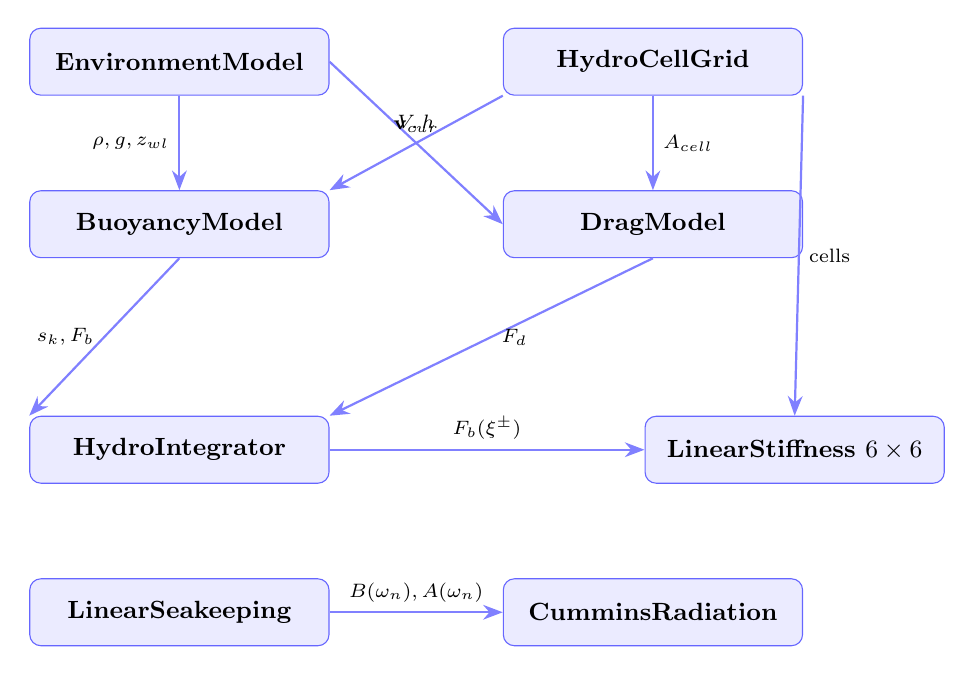
\begin{tikzpicture}[
  node distance=12mm and 22mm,
  mod/.style={rectangle, draw=blue!60, fill=blue!8, rounded corners=4pt,
              minimum width=3.8cm, minimum height=0.85cm,
              align=center, font=\small\bfseries},
  arr/.style={-{Stealth[length=2.5mm]}, thick, draw=blue!50},
]
\node[mod] (env)  {EnvironmentModel};
\node[mod, right=of env]  (grid) {HydroCellGrid};
\node[mod, below=of env]  (buoy) {BuoyancyModel};
\node[mod, right=of buoy] (drag) {DragModel};
\node[mod, below=20mm of buoy] (inte) {HydroIntegrator};
\node[mod, right=40mm of inte] (stif) {LinearStiffness $6\times6$};
\node[mod, below=of inte] (seek) {LinearSeakeeping};
\node[mod, right=of seek] (cumm) {CumminsRadiation};
\draw[arr] (env.south) -- (buoy.north) node[left,font=\scriptsize,midway]{$\rho,g,z_{wl}$};
\draw[arr] (env.east)  -- (drag.west) node[above,font=\scriptsize,midway]{$\mathbf{v}_{cur}$};
\draw[arr] (grid.south) -- (drag.north) node[right,font=\scriptsize,midway]{$A_{cell}$};
\draw[arr] (grid.south west) -- (buoy.north east) node[above,font=\scriptsize,midway]{$V,h$};
\draw[arr] (buoy.south) -- (inte.north west) node[left,font=\scriptsize,midway]{$s_k,F_b$};
\draw[arr] (drag.south) -- (inte.north east) node[right,font=\scriptsize,midway]{$F_d$};
\draw[arr] (grid.south east) -- (stif.north) node[right,font=\scriptsize,midway]{cells};
\draw[arr] (buoy.east |- stif.west) -- (stif.west) node[above,font=\scriptsize,midway]{$F_b(\xi^\pm)$};
\draw[arr] (seek.east) -- (cumm.west) node[above,font=\scriptsize,midway]{$B(\omega_n),A(\omega_n)$};
\end{tikzpicture}
\caption{Inter-model data dependency graph}
\label{fig:dependencies}
\end{figure}

\subsection{Computation Order (Each Step)}

\begin{enumerate}
  \item \textbf{Kinematics derivation:} Gazebo data $\to$ body-frame $\nuvec$, $\nudot$
  \item \textbf{Cell loop:} For each $k$:
        $d_k \to s_k \to F_{b,k}$ and $F_{d,k}$ $\to$ \texttt{AddWorldForce}
  \item \textbf{Hydrostatic stiffness:}
        $\xivec \to \Cvec\,\xivec$ $\to$ \texttt{AddWorldWrench}
  \item \textbf{Seakeeping / Cummins selection:}
    \begin{itemize}
      \item \textit{Cummins active:}
            $\nuvec \to I(t)$, $\nudot \to -\Ainf\nudot$, excitation separate $\to$ two wrenches
      \item \textit{Legacy mode:}
            $-\Avec\nudot - \Bvec\nuvec + F_{\text{exc}}$ $\to$ single wrench
    \end{itemize}
\end{enumerate}

\subsection{Force Budget}

\begin{table}[H]
  \centering
  \caption{Total force components}
  \begin{tabularx}{\linewidth}{lllX}
    \toprule
    \textbf{Component} & \textbf{Model} & \textbf{Profile} & \textbf{Physical Origin} \\
    \midrule
    $\Fvec_{\text{buoy}}$ & BuoyancyModel & all & Archimedes buoyancy \\
    $\Fvec_{\text{drag}}$ & DragModel & all & Viscous + form resistance \\
    $\Fvec_{\text{stiff}}$ & LinearStiffness & stiffness\_on & Hydrostatic restoring \\
    $\Fvec_{\text{rad}}$ & CumminsRadiation & cummins\_on & Radiation inertia + memory \\
    $\Fvec_{\text{exc}}$ & LinearSeakeeping & seakeeping\_on & Wave diffraction (1st order) \\
    \bottomrule
  \end{tabularx}
\end{table}

%% =======================================================================
\section{Coefficient Estimation Module -- \texttt{coeff\_estimator}}
%% =======================================================================

\subsection{Overview and Purpose}

\texttt{coeff\_estimator} is a Python utility package that automatically
computes all hydrodynamic coefficients required by the \texttt{usv\_hydro}
plugin from a given hull geometry.
It is located at
\texttt{usv\_sim\_ws/src/usv\_hydro/tools/coeff\_estimator/}
and can be run independently.

\textbf{Input}: Hull dimensions ($L$, $B$, $D$, $m$, $I_{xx}$, $I_{yy}$,
$I_{zz}$), or an SDF / STL file.

\textbf{Output}: A \texttt{hydro\_profiles.yaml} profile entry +
\texttt{seakeeping\_coeffs\_<name>.yaml}.

\subsection{Module Architecture}

\begin{table}[H]
  \centering
  \caption{\texttt{coeff\_estimator} module files}
  \begin{tabularx}{\linewidth}{lX}
    \toprule
    \textbf{File} & \textbf{Responsibility} \\
    \midrule
    \texttt{geometry\_loader.py}        & Converts SDF / STL / box parameters to a \texttt{ShipGeometry} object; derives $T$, $C_B$, $A_{wp}$, $S_{wet}$ \\
    \texttt{viscous\_drag\_estimator.py} & Computes $C_d$ via Hoerner (1965), $b_i$ via ITTC-1957, $A_{ii}$ via Lewis section method \\
    \texttt{bem\_solver.py}             & Produces $A(\omega)$, $B(\omega)$, $F_{\text{exc}}(\omega)$ via Capytaine BEM or closed-form Froude-Krylov \\
    \texttt{yaml\_writer.py}            & Writes results as a profile YAML entry and seakeeping coefficient YAML \\
    \texttt{estimate\_coeffs.py}        & CLI entry point (\texttt{box} / \texttt{sdf} / \texttt{stl} sub-commands) \\
    \bottomrule
  \end{tabularx}
\end{table}

\subsection{GeometryLoader -- Geometry Loader}

The \texttt{ShipGeometry} dataclass automatically derives the following:

\begin{align}
  T &= \frac{m}{\rho\,L\,B}
  &\text{(static equilibrium draft)} \label{eq:draft_calc}\\[4pt]
  C_B &= \frac{m/\rho}{L\,B\,T}
  &\text{(block coefficient)} \label{eq:cb_calc}\\[4pt]
  A_{wp} &= L\,B
  &\text{(waterplane area)} \label{eq:awp_calc}\\[4pt]
  S_{wet} &\approx 1.025\sqrt{V_{\text{disp}}\,L}
  &\text{(Denny-Mumford wetted surface)} \label{eq:swet_calc}
\end{align}

Automatic grid suggestion:
\begin{equation}
  N_x = \mathrm{clip}(\mathrm{round}(6L),\,4,\,20),\quad
  N_y = \mathrm{clip}(\mathrm{round}(6B),\,4,\,16),\quad
  N_z = 4
  \label{eq:grid_suggest}
\end{equation}

\subsection{ViscousDragEstimator -- Empirical Resistance}

\subsubsection{$C_d$ -- Hoerner Form Drag}

Hoerner (1965) form drag table with $C_B$ correction:

\begin{align}
  C_{d,x} &= 0.10 + 1.2\,(C_B - 0.50)^2
  &\text{(surge -- bow section)} \label{eq:cdx}\\[4pt]
  C_{d,y} &= 1.10 + 0.5\,(C_B - 0.60)
  &\text{(sway -- side surface)} \label{eq:cdy}\\[4pt]
  C_{d,z} &= 1.10 + \frac{0.8}{L/B}
  &\text{(heave -- bottom surface)} \label{eq:cdz}
\end{align}

\subsubsection{$b_x$ -- Surge Linear Damping (ITTC-1957)}

Reynolds number and ITTC-1957 friction coefficient:
\begin{align}
  Re &= \frac{V_{des}\,L}{\nu}, \qquad \nu = 1.14\times10^{-6}\;\text{m}^2/\text{s}
  \label{eq:re}\\[4pt]
  C_f &= \frac{0.075}{(\log_{10} Re - 2)^2}
  \label{eq:cf}
\end{align}

Frictional resistance and linear coefficient:
\begin{align}
  R_f &= \tfrac{1}{2}\rho\,V_{des}^2\,S_{wet}\,C_f\,(1+k_1)
  \label{eq:rf_est}\\[4pt]
  b_x &= \max\!\left(\frac{R_f}{V_{des}},\;\frac{m+A_{11}}{\tau_{\text{surge}}}\right)
  \label{eq:bx_est}
\end{align}

\subsubsection{$b_y$, $b_z$ -- Sway and Heave Damping}

From the heave critical damping ratio:
\begin{align}
  C_{33} &= \rho\,g\,A_{wp}
  \label{eq:c33_e}\\[4pt]
  \omega_{n,3} &= \sqrt{\frac{C_{33}}{m+A_{33}}}
  \label{eq:wn3}\\[4pt]
  b_z &= 2\,\zeta_{\text{heave}}\,\omega_{n,3}\,(m+A_{33})
  \label{eq:bz_e}
\end{align}

Sway with characteristic decay time:
\begin{equation}
  b_y = \frac{m+A_{22}}{\tau_{\text{sway}}},\qquad
  \tau_{\text{sway}} = \max\!\left(5.0,\;\frac{B}{2V_{des}}\right)
  \label{eq:by_e}
\end{equation}

\subsubsection{$A_{ii}$ -- Added Mass (Lewis Section)}

\begin{align}
  A_{11} &= \max(0.02,\;C_B-0.45)\,m
  &\text{(surge)}\\
  A_{22} &= \tfrac{\pi}{2}\rho\,(B/2)^2\,L\times 0.80
  &\text{(sway)}\\
  A_{33} &= \tfrac{\pi}{4}\rho\,(B/2)^2\,L\times 0.70
  &\text{(heave)}\\
  A_{44} &= 0.30\,I_{xx}
  &\text{(roll)}
  \label{eq:am_lewis}
\end{align}

\subsection{BEMSolver -- Wave Force Coefficients}

\subsubsection{Capytaine Mode (full BEM)}

When Capytaine is installed, a panel BEM solution is performed:
the hull mesh (box or STL) is generated, radiation and diffraction
problems are solved for each $\omega$, and $A(\omega)$, $B(\omega)$,
$F_{\text{exc}}(\omega)$ are assembled as $(6\times6)$ matrices.

\subsubsection{Empirical Mode (no Capytaine)}

Closed-form frequency-dependent models:

\begin{align}
  A_{ii}(\omega) &= A_{ii}^0 \cdot
    \frac{1 - \tanh\!\bigl((\omega-\omega_c)/\Delta\omega\bigr)}{2}
  \label{eq:a_emp}\\[4pt]
  B_{ii}(\omega) &= B_{\text{peak}} \cdot
    \exp\!\left(-\frac{(\omega-\omega_c)^2}{2\,\Delta\omega^2}\right)
  \label{eq:b_emp}
\end{align}

Froude-Krylov excitation forces:
\begin{align}
  F_{\text{exc},3} &= \rho g A_{wp}
  &\text{(heave, constant)}\\
  F_{\text{exc},1} &= i\,\rho g k\,V_{\text{disp}}
  &\text{(surge, inertia component)}\\
  F_{\text{exc},5} &= -F_{\text{exc},3}\,\frac{L\,k}{12}
  &\text{(pitch)}
  \label{eq:fexc_e}
\end{align}
where $k = \omega^2/g$ is the deep-water wave number.

\subsection{CLI Usage Examples}

\begin{lstlisting}
# 1. From box parameters (usv_minimal.sdf values)
python3 estimate_coeffs.py box \
    --L 2.2 --B 1.1 --D 0.5 --mass 350 \
    --ixx 42.58 --iyy 148.46 --izz 176.46 \
    --name usv_minimal --out output/ --bem

# 2. Automatic read from SDF
python3 estimate_coeffs.py sdf \
    --sdf ../usv_description/sdf/usv_minimal.sdf \
    --name usv_minimal --out output/

# 3. STL mesh + full BEM (Capytaine required)
python3 estimate_coeffs.py stl \
    --stl hull.stl --mass 350 --bem \
    --omega-min 0.3 --omega-max 3.14 --n-omega 12 \
    --name my_hull --out output/
\end{lstlisting}

\subsection{Reference Vessel Results}

The table below compares estimation results obtained with
\texttt{usv\_minimal.sdf} ($2.2\times1.1\times0.5$ m, 350 kg)
against the \texttt{baseline} profile values in \texttt{hydro\_profiles.yaml}.

\begin{table}[H]
  \centering
  \caption{Estimated vs.\ baseline profile values}
  \begin{tabular}{lccc}
    \toprule
    \textbf{Quantity} & \textbf{Estimated} & \textbf{baseline} & \textbf{Note} \\
    \midrule
    $C_{d,x}$ (surge) & 0.343 & 0.90 & Low for $C_B{=}1$; expected \\
    $C_{d,y}$ (sway)  & 1.275 & 1.30 & Consistent \\
    $C_{d,z}$ (heave) & 1.500 & 2.00 & Conservative estimate \\
    $b_x$ [N$\cdot$s/m] & 18.1 & 18.0 & Nearly identical \\
    $b_y$ [N$\cdot$s/m] & 237  & 55   & Large Lewis $A_{22}$ contribution \\
    $b_z$ [N$\cdot$s/m] & 1237 & 80   & $\zeta{=}0.15$ + high $C_{33}$ \\
    \midrule
    Static draft $T$ & 0.1446 m & 0.145 m & $<0.05\%$ error \\
    $A_{wp}$ & 2.42 m$^2$ & 2.42 m$^2$ & Exact \\
    $F_{exc,3}$ (heave) & 23\,740 N/m & 23\,738 (analytical) & $<0.01\%$ \\
    \bottomrule
  \end{tabular}
\end{table}

\begin{table}[H]
  \centering
  \caption{Empirical added mass estimates}
  \begin{tabular}{lrl}
    \toprule
    \textbf{DOF} & \textbf{Value} & \textbf{Unit} \\
    \midrule
    $A_{11}$ surge  & 192.5  & kg \\
    $A_{22}$ sway   & 836.3  & kg \\
    $A_{33}$ heave  & 365.9  & kg \\
    $A_{44}$ roll   & 12.77  & kg$\cdot$m$^2$ \\
    $A_{55}$ pitch  & 129.83 & kg$\cdot$m$^2$ \\
    $A_{66}$ yaw    & 44.12  & kg$\cdot$m$^2$ \\
    \bottomrule
  \end{tabular}
\end{table}

%% =======================================================================
\section{Configuration Guide}
%% =======================================================================

\begin{lstlisting}
defaults:
  fluid_density: 1000.0     # [kg/m^3]
  gravity: 9.81             # [m/s^2]
  water_level: 0.0          # [m]
  link_name: "hull_link"
  cells: [14, 8, 4]
  cd: [0.9, 1.3, 2.0]
  drag:
    linear_total: [18.0, 55.0, 80.0]
    scale_by_cell_count: true

profiles:
  stiffness_on:
    hydrostatic_stiffness:
      enabled: true
      scale: 1.0
      heave_step: 0.01       # [m]
      angle_step: 0.001      # [rad]

  cummins_on:
    linear_seakeeping:
      enabled: true
      coeffs_file: "seakeeping_coeffs_example.yaml"
      excitation_omega: 0.8  # [rad/s]
      excitation_scale: 1.0
    cummins_radiation:
      enabled: true
      kernel_max_t: 20.0     # [s]
      kernel_dt: 0.0         # 0 = use sim step
\end{lstlisting}

%% =======================================================================
\section{Testing and Validation}
%% =======================================================================

\begin{table}[H]
  \centering
  \caption{Unit test coverage (21/21 passed, 3.04 s)}
  \begin{tabularx}{\linewidth}{llX}
    \toprule
    \textbf{Test Suite} & \textbf{Count} & \textbf{Validated} \\
    \midrule
    \texttt{BuoyancyModelTest}         & 3 & Archimedes, partial submergence, equilibrium draft \\
    \texttt{DragModelTest}             & 3 & Current damping, linear/quadratic components \\
    \texttt{HydroScenarioTest}         & 6 & Equilibrium, roll/pitch moment, $C_{11}/C_{22}\approx0$, $C_{35}\approx C_{53}$ \\
    \texttt{CumminsRadiationModelTest} & 6 & Kernel construction, zero-velocity test, $A(\infty)$, memory accumulation \\
    \texttt{HydroConfigTest}           & 3 & YAML validation \\
    \bottomrule
  \end{tabularx}
\end{table}

%% =======================================================================
\section{Current Limitations and Development Roadmap}
%% =======================================================================

\subsection{Current Limitations}

\begin{itemize}
  \item AABB-based box hull approximation; no true cross-sectional geometry
  \item Single harmonic wave; irregular sea states (JONSWAP) not supported
  \item No Munk moment, cross-flow lift
  \item No propulsion or rudder model
\end{itemize}

\subsection{Phase 2 -- MMG Manoeuvring Model}

\begin{align}
  N_{\text{Munk}} &= -\tfrac{1}{2}\rho(m_{11}-m_{22})uv \label{eq:munk} \\
  Y_{cf} &= -\tfrac{1}{2}\rho C_{dL}\,L\,d\,|v|v \label{eq:crossflow} \\
  T &= \rho n^2 D^4 K_t(J),\quad J = \frac{u(1-w)}{nD} \label{eq:propeller}
\end{align}

%% =======================================================================
\appendix
\section{Symbol List}
%% =======================================================================

\begin{table}[H]
  \centering
  \begin{tabularx}{\linewidth}{llX}
    \toprule
    \textbf{Symbol} & \textbf{Unit} & \textbf{Definition} \\
    \midrule
    $\rho$ & kg/m$^3$ & Fluid density \\
    $g$ & m/s$^2$ & Gravitational acceleration \\
    $\mathbf{R}$ & -- & Rotation matrix \\
    $\nuvec\in\mathbb{R}^6$ & m/s, rad/s & Body-frame 6-DOF velocity \\
    $\nudot\in\mathbb{R}^6$ & m/s$^2$ & Body-frame 6-DOF acceleration \\
    $\xivec\in\mathbb{R}^6$ & m, rad & 6-DOF displacement \\
    $s_k$ & -- & Submergence fraction $[0,1]$ \\
    $V_{\text{cell}}$ & m$^3$ & Cell volume \\
    $d_k$ & m & Cell depth \\
    $b_i$ & N$\cdot$s/m & Linear damping \\
    $C_{d,i}$ & -- & Morison drag coefficient \\
    $\Cvec\in\mathbb{R}^{6\times6}$ & N/m & Hydrostatic stiffness \\
    $\Avec(\omega)$ & kg & Added mass matrix \\
    $\Bvec(\omega)$ & N$\cdot$s/m & Radiation damping matrix \\
    $\Ainf$ & kg & Added mass at infinite frequency \\
    $\Kvec(t)$ & N$\cdot$s/m$^2$ & Retardation kernel \\
    $T_{\max}$ & s & Cummins memory window \\
    $\Delta t_k$ & s & Kernel time step \\
    $C_B$ & -- & Block coefficient \\
    $A_{wp}$ & m$^2$ & Waterplane area \\
    $S_{wet}$ & m$^2$ & Wetted surface area \\
    $T$ & m & Static draft \\
    $k$ & 1/m & Deep-water wave number $\omega^2/g$ \\
    \bottomrule
  \end{tabularx}
\end{table}

\section{Reference Vessel Parameters}

\begin{table}[H]
  \centering
  \begin{tabular}{lll}
    \toprule
    \textbf{Parameter} & \textbf{Value} & \textbf{Unit} \\
    \midrule
    $L \times B \times D$ & $2.2\times 1.1\times 0.5$ & m \\
    Mass $m$ & 350 & kg \\
    $I_{xx}$ & 42.58 & kg$\cdot$m$^2$ \\
    $I_{yy}$ & 148.46 & kg$\cdot$m$^2$ \\
    $I_{zz}$ & 176.46 & kg$\cdot$m$^2$ \\
    $\rho$ & 1000 & kg/m$^3$ \\
    Static draft & 0.145 & m \\
    $A_{wp}$ & 2.42 & m$^2$ \\
    \bottomrule
  \end{tabular}
\end{table}

\vfill
\begin{center}
  \small\textcolor{gray}{
  This report is generated from \texttt{usv\_hydro} source code.
  Phase 1 complete -- 21/21 tests passed.
  }
\end{center}

\end{document}
